% !TeX spellcheck = fr_FR
\chapter{Rapport d'audit fonctionnel et technique}
\label{annexe_A_rapport_audit}

\section*{Introduction}
\addcontentsline{toc}{section}{Introduction} 

\subsection*{Contexte} 
\addcontentsline{toc}{subsection}{Contexte}
A l’origine, la bibliothèque Cujas a été créée en 1829 pour desservir la bibliothèque de la Faculté de droit de Paris. En 1970, elle devient une bibliothèque interuniversitaire à la suite des réformes universitaires1. Cujas est spécialisée en droit, en économie et en sciences politiques, elle constitue aujourd’hui une bibliothèque de référence nationale et internationale dans ces domaines2. Par ailleurs, elle devient pôle associé de la BnF en sciences juridiques. 

En 1979, elle devient bibliothèque interuniversitaire par convention entre les universités de Panthéon-Sorbonne (Paris I) et Panthéon-Assas (Paris II)3. Elle possède un riche patrimoine documentaire plus de 40 000 volumes anciens et un fonds francophone et international d’une grande diversité4. 

La bibliothèque possède aussi des fonds spécialisés. Elle conserve un ensemble unique de collections de sciences juridiques, économique et politiques  : thèses et mémoires, publications officielles de la Société des Nations, des Nations Unies, Journal officiel de la France et des anciennes colonies. Elle conserve également une collection de travaux académiques imprimés en Allemagne aux XVIe et XIXe siècle, des documents retraçant la sociabilité universitaire et l’histoire de l’enseignement de l’ancienne Faculté de Droit de Paris5. 

Entre 2001 et 2004, la bibliothèque Cujas entreprend une première phase de numérisation autour d’un projet d’exposition virtuelle pour le bicentenaire du Code civil (2004) confiant cette prestation à la société Safig. Il s’agit alors d’une numérisation en mode image et en niveaux de gris, avec une saisie manuelle de la table des matières ou au moins de la pagination. Le prestataire fournit l’hébergement des données6. 



\subsection*{Présentation du projet de la bibliothèque} 
\addcontentsline{toc}{subsection}{Présentation du projet de la bibliothèque}

En 2006, la décision est prise de créer une bibliothèque numérique juridique, à l’origine du projet de CujasNum. Deux enseignants-chercheurs, Laurent Pfister et Franck Roumy, rédigent une liste de « fondamentaux du droit » à numériser en priorité : 471 ouvrages du XVe au XXe siècle, soit 1 462 volumes et environ 1 001 559 pages issus de la réserve Pavillon7. 

A l’origine, la BIU Cujas souhaite devenir un pôle de réplication de Persée et acquiert un scanner Kirtas pour ce projet. Toutefois, sa candidature n’est pas retenue. Elle refond alors son projet en diminuant le nombre d’ouvrages à numériser et en se coordonnant avec la BnF qui a créé sa propre liste de fondamentaux du droit, la liste Kerbrat8.  

La liste Pfister-Roumy retravaillée est constituée de près de 435 titres des XVème au XXème siècles qui sont des fondamentaux de l’histoire du droit : sources normatives en droit romain, en droit coutumier, en législation, jurisprudence et doctrine9. 

L’enjeu de la bibliothèque numérique est de favoriser l’étude et la recherche en sciences juridiques, en facilitant l’accès à l’information, d’apporter du contenu au système d’information de la bibliothèque afin qu’il devienne un outil de travail performant pour l’ensemble des publics intéressés. Il est nécessaire également de protéger les collections de la BIU Cujas tout en accroissant leur utilisation, de les valoriser en les rendant accessibles plus facilement en France et à l’étranger, augmentant ainsi la visibilité du droit français10. 

CujasNum est développée sous XTF. Il s’agit au début d’un catalogue de PDF accessible en ligne avec des tables des matières écrites manuellement permettant de naviguer à l’intérieur du document11. En 2013, l’implémentation d’une visionneuse JPEG permet aux usagers de consulter les documents directement dans la bibliothèque numérique12. Quoique robuste, XTF est devenu obsolète avec le temps et répond difficilement aux besoins actuels des usagers (impossibilité d'éditorialiser les collections ou d'intégrer d’autres types de documents).  

Face à ce constat, un nouveau prototype interne est actuellement à l’étude. L’enjeu de cette refonte est de sortir la bibliothèque numérique de son isolement en la faisant basculer vers un outil ouvert et interopérable (via l’intégration de serveurs IIIF, d’API et du protocole OAI-PMH), afin de pouvoir s’insérer dans les grands projets documentaires nationaux de l’Enseignement Supérieur, tels que le projet Orion de l’Abes13. 

\subsection*{Méthodologie employée}
\addcontentsline{toc}{subsection}{Méthodologie employée}

Cette étude se déroule entre le 1er avril et le 31 juillet 2026. Les avis et les besoins liés à l’existant ont été obtenu entre croisant différentes méthodes : des entretiens avec les professionnels de Cujas et les enseignants-chercheurs, des échanges informels ainsi qu’une enquête en ligne qui a eu lieu du 14 avril au 3 juillet 2026. 

Ces éléments sont complétés par mes propres observations et analyses. Mes recommandations sont toutefois renvoyées au document de préconisation ciblées que je livrerai à l’issue de ce stage. 

\subsection*{Objectifs des entretiens}  
\addcontentsline{toc}{subsection}{Objectifs des entretiens}

L’objectif de ces entretiens menés sont multiples. D’abord, il s’agit de disposer d’un retour critique sur la bibliothèque numérique actuelle, de comprendre les attentes des chercheurs, et des services de la BIU Cujas concernant la future bibliothèque numérique, en particulier en terme de fonctionnalités et de services. Cela permet de disposer d’éléments pour préparer des propositions fonctionnelles pour le projet. 


\section*{Analyse fonctionnelle} 
\addcontentsline{toc}{section}{Analyse fonctionnelle}

\section{Les contenus} 

\subsection{L’analyse de l’existant}

\subsubsection{La politique documentaire et la qualité scientifique des contenus} 

Les chercheurs signalent une lacune importante dans les collections numérisées concernant les recueils de la période 1930 à 1980. Ce manque est lié aux contraintes du domaine public empêchant la diffusion libre de bon nombre d’ouvrages numérisés de cette période ainsi qu’à la date déjà ancienne de création de la liste Pfister-Roumy. Ces lacunes pourraient cependant être en partie comblées par la négociation d’accords ou un dispositif technique, comme le font d’autres établissements14. 

\subsubsection{La diversité des types de documents} 

	Actuellement, la bibliothèque numérique propose uniquement des monographies15. Cette situation génère une forte insatisfaction tant du côté du Département du patrimoine, de la conservation et de la numérisation (DPCN) que de celui du Département des Périodiques et des ressources électroniques (DPRE). La cause principale est d’ordre technique. En effet, le logiciel sous XTF de CujasNum accepte uniquement l’arborescence « à plat » empêchant ainsi l’intégration de documents nécessitant une hiérarchie16, comme les revues ou les archives. Ils ne peuvent pas pour le moment intégrer ou traiter d’autres formats comme des périodiques qui nécessitent une architecture arborescente17.

\subsubsection{L’éditorialisation} 

L’éditorialisation des contenus par le DPCN est actuellement impossible sous XTF sans une intervention du Département informatique technique. L’absence d’outils d’éditorialisation empêche la création de corpus spécifiques et limite la finesse d’affichage18. L’éditorialisation se résume donc à une présentation sommaire des corpus, une production de tables de matières et une structuration en collections chronologiques ou thématiques. 

Les utilisateurs qualifient l’organisation actuelle des collections de « casse-tête » chronophage19. Le mélange entre des collections thématiques et chronologiques n’est pas intuitif, et les vignettes présentes sur la page d’accueil créent de fausses attentes quant à la précision des sources proposées20.  

La bibliothèque numérique actuelle n’est pas rattachée aux canaux de communication existant dans la bibliothèque Cujas. Actuellement, CujasNum ne partage aucune nouveauté concernant les numérisations misent en ligne sur le site, participant ainsi à son invisibilité auprès des utilisateurs21. Il existait auparavant un bulletin de numérisation22 qui jouait ce rôle de communication avec les lecteurs mais qui a été arrêté au moment du COVID.   

\subsubsection{L’intégration de collections d’autres bibliothèques numériques} 

L’infrastructure actuelle souffre d’un fort isolement. Bien qu’il existe un partenariat de numérisation avec Persée pour les revues scientifiques et juridiques, les fichiers générés ne sont pas disponibles et ne peuvent actuellement pas être reversés ou rapatriés dans le système de la bibliothèque Cujas23. Il est également impossible de rapatrier les contenus numérisés et consultés massivement sur le portail de la BNF à cause de blocages architecturaux24. Il n’est pas non plus possible de rapatrier dans la bibliothèque numérique un volume lacunaire qui aurait été numérisé par un autre établissement. 

\subsection{Les propositions d’améliorations des répondants}

\subsubsection{La politique documentaire et la qualité scientifique des contenus}

Pour pallier les manques actuels, il est recommandé de compléter les numérisations de la période 1800 à 1940, notamment pour les manuels de droit civil, de procédure et de droit commercial25. Il serait également pertinent de numériser les différentes éditions successives d’un même ouvrage afin de permettre aux chercheurs de retracer l’évolution de la pensée d’un auteur au fil du temps. Pour piloter cette politique documentaire, la création d’un comité scientifique est suggérée pour établir des priorités de numérisation de façon collaborative comme ce fut le cas pour la liste Pfister-Roumy26.  

\subsubsection{La diversité des types de documents}

L’amélioration technique majeure attendue est la capacité d’accueillir de nouveaux types de documents pour refléter la richesse des collections de Cujas27. Le système devra impérativement prendre en charge les revues et les périodiques ainsi que les documents iconographiques et les archives28. Cela permettrait de mettre davantage en avant la richesse des collections de Cujas. Il s’agit d’un souhait évoqué par les chercheurs et les différents services de la bibliothèque.  

\subsubsection{L’éditorialisation} 

C’est l’un des besoins les plus fortement exprimés pour redonner de la cohérence aux collections. Il est préconisé d’ajouter des textes explicatifs et scientifiques pour justifier la logique de classification adoptée, évitant ainsi la confusion des utilisateurs face à des regroupements thématiques ou chronologiques d’apparence incohérente29. L’éditorialisation doit être pensée par des juristes pour des juristes, afin d’expliquer concrètement pourquoi un ouvrage est important pour l’histoire du droit30. Plusieurs formats sont proposés :  

La création de parcours thématiques guidés ou d’une « galerie des grands juristes »31, proposant des notices biographiques et des liens directs vers leurs œuvres32. 

L’intégration d’explications sur le contexte de publication (privilèges accordés, choix des éditeurs, évolution de la doctrine au fil des rééditions)33.  

L’organisation des contenus en sous-catégories claires et rationnelles (droit, doctrine, revues, jurisprudence)34. 

\subsubsection{Les éléments de communication} 

Pour valoriser la bibliothèque numérique et accompagner ses publics, il est proposé de créer des supports explicatifs, comme des vidéos de présentation de corpus35. Proposer des retours d’expérience concrets (par exemple, un doctorant détaillant la procédure suivie pour prendre en main la bibliothèque afin de préparer son article) constituerait une excellente porte d’entrée pour transmettre des conseils d’utilisation (tips) aux nouveaux chercheurs36. L’ajout de tutoriels ou de foire aux questions seraient une aide supplémentaire pour prendre en main la bibliothèque numérique pour les nouveaux utilisateurs ou mêmes les plus anciens afin d’avoir un document de référence lorsqu’ils sont confrontés à de nouveaux outils ou services37.  

\subsubsection{L’intégration de collections d’autres bibliothèques numériques}

La bibliothèque numérique doit s’affranchir de son isolement actuel pour devenir un véritable portail interconnecté38. Plutôt que de numériser ce qui existe déjà, le nouveau système doit être en mesure de moissonner et rapatrier les données d’autres institutions, de créer des ponts et des liens externes vers des plateformes comme Persée ou Dalloz39. Elle doit pouvoir être capable de reconstituer virtuellement les corpus dispersés de la liste Pfister-Roumy40.  



\section{Les publics}

\subsection{L’analyse de l’existant} 

\subsubsection{Les profils des utilisateurs}

A l’origine de la création de CujasNum, le public cible était les chercheurs. Cujas étant une bibliothèque de recherche, la bibliothèque numérique a donc été développée pour répondre à leurs besoins41. 

Au fil du temps, le public consultant la bibliothèque numérique s’est étoffé d’autres visiteurs comme les doctorants et les étudiants en droit et en histoire du droit. Les résultats de l’enquête vont dans ce sens aussi. 18.52\% des répondants sont étudiants, 19.75\% des enseignants ou des chercheurs, 32.10\% des professionnels de l’information et des bibliothèques, et 9.88\% des doctorants. Les professionnels du droit ne représentent à ce jour que 2.47\% des répondants42.  

Une grande partie du public est spécialisé en droit (43.10\%), mais on observe que le reste de l’audience se divise en plusieurs domaines de spécialité dont deux relativement proches. Les spécialistes de l’histoire du droit (9.88\% des répondants) et les spécialistes en histoire (8.64\% des répondants). Ils sont suivis de près par les historiens du livre ou de l’édition (7.41\%). Une minorité de répondants ont pour domaine de spécialité l’économie ou la statistique (2.47\%). 7.4\% ont une autre spécialité43. 

\subsubsection{La fréquentation}

L’attrait des chercheurs pour la bibliothèque numérique de Cujas vient de la richesse de ses collections, principalement en histoire du droit. Les chercheurs apprécient de la consulter, car ils ont accès à des documents qu’il leur serait compliqué ou fastidieux de trouver et consulter sans elle44. 

Les chercheurs privilégient une bibliothèque numérique à une autre en raison de son programme de numérisation. Ils savent que lorsqu’ils consultent les collections de Cujas ils trouveront principalement les sources de droit : le contenu de CujasNum est donc bien identifié par ses lecteurs45.  

\subsubsection{Les statistiques de consultation}

La bibliothèque numérique a perdu en visibilité. Cette cause est liée à plusieurs facteurs. Il se trouve qu’on la voit difficilement sur la page d’accueil du site de Cujas46. On est obligé de faire défiler la page pour la trouver et elle n’apparait pas dans les onglets du site de la bibliothèque Cujas47. Lorsque l’on fait une recherche dans un moteur de recherche comme celui de Google, le PageRank est mauvais. La recherche d’un titre n’arrive \enquote{qu’en cinquième ou sixième pages de résultats}48.  

\subsection{Les propositions d’améliorations des répondants}

Les différents services de la bibliothèque se retrouvent autour de l’importance d’élargir le public cible de la future bibliothèque numérique et de ne plus se cantonner uniquement à celui des chercheurs. Il est primordial pour la bibliothèque d’intégrer dans le public visé le grand public49. En élargissant son public, cela lui permettrait de répondre à son objectif qui est de rendre la bibliothèque à terme capable d’agréger le contenu d’autres bibliothèques politiques ou juridiques devenant ainsi une plateforme pour les bibliothèques de droit50. Dans un objectif à long terme, Cujas aimerait devenir une alternative et un pôle de référence pour les juristes51.  

Pour la direction, il est important de faire en sorte d’alléger la charge de travail en exploitant les nouveaux outils d’automatisation basée sur les données (IA, extraction depuis XML-ALTO). Ce n’est pas parce que le \enquote{monde des juristes} a commencé à traiter la question que les bibliothèques ne peuvent pas s’y pencher eux aussi. Il est important que le personnel de la bibliothèque y soit formé afin de comprendre comment ces outils sont exploités et fonctionnent52. 



\section{La description des documents}

\subsection{L’analyse de l’existant}

Actuellement, les notices bibliographiques sont incomplètes et accessibles uniquement sous la forme d’infobulles.  Les notices sur les livres anciens sont souvent pauvres. Avant 2013, les standards et les normes de catalogage du livre ancien n’étaient pas utilisés à Cujas.  

On trouve également deux versions des notices bibliographiques qui sont plus ou moins renseignées en fonctions de l’endroit où elles sont consultées53. La version accessible depuis la liste de résultats est \enquote{plus détaillée} que celle à partir de la visionneuse54.  

Il manque l’affichage d’une page dédiée à chaque document permettant à l’utilisateur d’avoir un aperçu clair des informations55. A son stade de développement, le prototype propose cette page. En effet, à l’intérieur du prototype chaque document possède sa propre page avec une distinction claire de chaque élément constituant la notice permettant à l’utilisateur de repérer les éléments qui l’intéressent. Toutefois, certains problèmes repérés sur CujasNum y demeurent identiques56.  

Par ailleurs, aucun des éléments écrits dans la notice n’est relié ou adossé à un référentiel57. Il n’est pas possible de faire des rebonds auteur ou sujet. Il n’est pas non plus possible de créer des liens vers la notice papier ou vers des sites se trouvant à l’extérieur de la bibliothèque58.  

Enfin, la notice affichée à partir de la visionneuse est indiquée comme étant complète alors que la notice la plus complète est celle que l’on peut afficher dans la liste de résultat ou bien à partir des vignettes59.  

\subsection{Les propositions d’amélioration des répondants} 

Les notices bibliographiques de la future bibliothèque numérique doivent être adossées à des référentiels. Un alignement des métadonnées doit être effectué dans ce sens. Cela permettrait de faire rapprochement entre les documents mais aussi entre les différentes collections à travers la création de rebonds auteurs ou sujets60.  

Il faudrait également avoir la possibilité de \enquote{paramétrer les éléments de la Dublin Core} s’affichant sur le portail de la bibliothèque numérique61. Dans l’idéal, il serait bien que la description du document puisse contenir l’indexation Rameau ainsi que celle propre à la bibliothèque Cujas. Un des souhaits mentionnés par les utilisateurs est de savoir s’il est possible d’avoir un titre abrégé en français notamment pour les documents en latin afin de permettre au non-spécialiste d’avoir une idée de ce dont traite le document63.  



\section{La recherche d’information}

\subsection{L’analyse de l’existant}

\subsubsection{Les moyens de recherche : recherche simple, avancée et dans l’OCR}

Les utilisateurs et les différents services sont enclins à dire que la recherche simple fonctionne relativement bien. La troncature et la recherche par mots-clés satisfait les utilisateurs qui trouvent utile le petit guide écrit en-dessous de la barre de recherche permettant d’avoir une compréhension rapide de son utilisation.  

En revanche, l’avis est plus négatif concernant la recherche avancée, en particulier des personnels de la bibliothèque. De plus, une confusion peut être faite entre la recherche plein-texte et celle avancée. Ces deux recherches se trouvent sur la même page pouvant laisser croire qu’ils fonctionnent de la même façon. La recherche plein-texte ne peut être utilisée à son plein potentiel étant donné que de nombreux documents numérisés ne sont pas océrisés. L’absence d’OCR, très demandé par les chercheurs les amène à contourner cette difficulté en faisant appel à leurs frais à des outils comme Abode Pro pour le générer eux-mêmes64. 

Les chercheurs utilisent énormément la navigation dans la table des matières. Ils soulignent l’importance de celles-ci car cela leur permet d’économiser du temps de recherche. Ils apprécient d’avoir la possibilité de pouvoir cliquer sur une section ou une sous-section dans le document et de s’y rendre directement65. Les tables des matières rendent le document numérisé plus manipulables, et permettent un usage proche de celui d’un livre papier66. 

\subsubsection{Navigation par thèmes}  

Les utilisateurs expriment leur mécontentement concernant la navigation par thèmes qu’ils trouvent incohérente. Ils ne comprennent pas la manière dont été constitué les collections et soulignent le manque d’explication pour comprendre la logique utilisée pour répartir les documents67. 

L’organisation actuelle, qui mélange des collections thématiques et chronologiques, pose plusieurs problèmes. Par exemple, la présence d’un auteur du XVIIe siècle dans la collection du droit romain crée une incohérence chez les historiens du droit qui associent ce type de droit à l’Empire romain68. 

Les titres des collections sont à la fois trop précis et trompeurs et ne correspondent pas au contenu réel de chacune des collections69.  

Les filtres et les facettes proposés dans la bibliothèque numérique ne répondent plus aux besoins des utilisateurs qui s’en plaignent et rejoignent sur ce point le mécontentement des services internes de Cujas notamment le DPCN. Les facettes utilisées dans CujasNum sont issues d’une indexation propre à la bibliothèque Cujas. Cette indexation déconstruit l’indexation RAMEAU lorsque ce langage ne permet pas une description satisfaisante des documents de la bibliothèque numérique70. 

Les filtres générés par cette indexation sont trop précis (nombre d’entre eux ne sont liés qu’à un seul document), contraignant l’utilisateur dans sa recherche71. On remarque une forte répétition des mêmes facettes amenant à rendre cette indexation illisible. L’utilisateur ne parvient pas à voir quel filtre il a sélectionné car celui-ci ne se distingue pas dans la masse des filtres existant72. Certaines des indexations contiennent le nom d’un ouvrage important de l’histoire du droit : les chercheurs soulignent l’inutilité de cette indexation quand une recherche par titre suffit pour trouver le document73.  

\subsection{Les propositions d’amélioration des répondants}

\subsubsection{Les moyens de recherche : recherche simple, avancée et par OCR}

Une forte demande a été exprimée par les chercheurs concernant la recherche plein-texte. Ils insistent en particulier sur la nécessité de disposer à la fois d’une recherche plein texte et de tables des matières ce qui constitue un véritable atout pour mener leurs recherches dans de bonnes conditions74. Ces deux éléments permettent une manipulation du document numérique proche de celle du livre papier75.  

Il serait apprécié qui soit signalé, par exemple dans la notice, le taux d’océrisation réelle des documents. Par ailleurs, de nombreux documents ont été océrisés sans que cela ne soit signalé dans la notice. Cette mention devrait figurer sur la page du document afin que l’on puisse filtrer la liste de résultats pour ne conserver que les documents océrisés76. 

\subsubsection{Navigation par thèmes}  

Actuellement, les collections sont créées grâce à des requêtes77. Il serait nécessaire de proposer un autre modèle de construction de collection pour permettre la création de collection et de sous-collection à l’intérieur de celle-ci tout en ajoutant de l’éditorialisation pour justifier les choix78. Pour les chercheurs, aucune constitution n’est mauvaise en soi tant qu’elle peut être justifiée et expliquée79. 

\subsubsection{Filtres et facettes} 

Les filtres et les facettes doivent être plus généraux et regrouper plusieurs documents. Il serait également important que celles-ci puissent adaptées aux différents types de documents numérisés, surtout si l’on souhaite ajouter des périodiques. Un filtre trop précis n’est pas forcément pertinent pour ce type de contenu80.  

Il peut être utile d’avoir des facettes mieux constituées, proposant une arborescence claire à plusieurs niveaux (exemple donné : une entrée code peut être déclinée en code français et code étranger)81.  



\section{La consultation} 

\subsection{L’analyse de l’existant}

Dans CujasNum, la visionneuse JPEG fonctionne bien et est de bonne qualité. Elle permet d’intégrer la table des matières en prenant en compte l’arborescence complète. Elle peut aller jusqu’à sept niveaux82. La table des matières, cliquable directement dans la visionneuse ainsi qu’à l’intérieur du PDF, constitue une aide à la recherche grandement appréciée par les chercheurs83. 

Dans le prototype, on observe que plusieurs visionneuses ont été mises à dispositions ce qui est un avantage certain pour élargir le public de la bibliothèque numérique. Le lecteur peux choisir entre une visionneuse simple d’utilisation comme UniversalViewer ou une plus technique comme Mirador84. Cela laisse l’utilisateur libre de choisir ses modalités de consultation et s’adapte à ses besoins et compétences.  

Toutefois, dans le prototype, on remarque que Mirador a du mal à afficher la table des matières, en raison du niveau d’arborescence et de caractères possibles trop restreints85. 

Les chercheurs sont satisfaits de pouvoir télécharger le document sous format PDF86. C’est un format que tous connaissent et apprécient. 

\subsection{Les propositions d’amélioration des répondants}

Les chercheurs aimeraient avoir la possibilité de pouvoir comparer deux documents sur la même interface, ou d’extraire une partie du texte qui les intéresse afin de le mettre dans leurs cours87.  

Ils sont nombreux à souhaiter être en mesure de ne télécharger qu’une partie du document et de sélectionner les pages qu’ils souhaitent88. Le cas échéant, il serait apprécié de pouvoir conserver la page de garde de l’ouvrage afin de savoir d’où l’information a été extraite89.  

Les chercheurs apprécieraient de disposer de la référence bibliographique complète de l’ouvrage. Cela leur ferait gagner du temps en ayant simplement à faire un copier-coller dans leur document90. 



\section{Les services proposés}

\subsection{L’analyse de l’existant}

Actuellement, peu de services sont proposés dans la bibliothèque numérique. La bibliothèque ne propose pas de compte personnel permettant d’enregistrer son historique de recherche, ou de mettre en favoris des ouvrages numérisés. Il est également impossible d’exporter une référence bibliographique91. 

En principe la bibliothèque numérique permet de se constituer un panier de recherche constitué de favoris que l’on peut s’envoyer par mail sous forme de liste. Cependant, la liste ne parvint pas à être envoyé à cause d’une « erreur de servlet inattendue ». La connexion est refusée rendant impossible l’envoi de la liste d’ouvrage sélectionné92.  

Par ailleurs, il n’est pas possible de conserver l’historique des requêtes de recherche ou d’ajouter des libellés afin de regrouper les documents traitant d’un sujet identique. Un autre problème est la perte des favoris collectés par les lecteurs lorsque l’on ferme la page du site. Le panier ne garde pas en mémoire les favoris93. Les lecteurs ne perçoivent donc pas l’intérêt de ce service.  

\subsection{Les propositions d’amélioration}

L’enquête en ligne a démontré que parmi les différents services proposés, celui d’avoir un compte personnel ressort. Nombreux sont les répondants qui aimeraient avoir la possibilité de pouvoir enregistrer en favoris les ouvrages consultés, tout en permettant de se créer une arborescence avec des fichiers afin de les classer94. Pour une majorité, le compte personnel n’a pas besoin d’être très sophistiqué et peut proposer des fonctionnalités simples95.  

Les personnels de Cujas et les lecteurs se rejoignent sur l’utilité de disposer d’un compte personnel dans la bibliothèque numérique. Il faudrait que celui-ci permette de mettre en favoris les ouvrages, d’enregistrer les requêtes, d’avoir un historique de recherche et de pouvoir faire  une recherche uniquement dans les favoris. Le compte personnel devrait aussi donner la possibilité de partager des documents et de paramétrer des notifications afin d’être alerté lors de la mise en ligne d’un ouvrage susceptible d’intéresser96.  

La direction aimerait beaucoup qu’il soit possible avec la refonte de la bibliothèque numérique de pouvoir mettre en place des services plus avancées permettant la fouille de texte. Elle propose pour ce faire de s’appuyer sur les ressources d’ISTEX. Par exemple, on pourrait permettre à travers une requête SQL, la création d’un corpus de document généré à la volée97 pour les chercheurs qui souhaitent réaliser une fouille de textes.   

Enfin, un enseignant-chercheur recommande de mettre en avant la bibliothèque numérique Cujas à travers les réseaux sociaux afin de rendre la bibliothèque davantage visible98.  



\section{Ergonomie}

\subsection{L’analyse de l’existant}

Le prototype et CujasNum partagent, à quelques exceptions près, la même présentation générale des éléments. Cette architecture similaire permet à l’utilisateur de comprendre rapidement les sources disponibles. Toutefois aucun plan du site n’est accessible depuis la page d’accueil. 

Dans le prototype, certaines fonctionnalités sont répétées ou subdivisées en plusieurs endroits ce qui nuit à leur visibilité. C’est le cas de la fonction de recherche, présente en plusieurs endroits avec des modalités différentes pas toujours compréhensibles :  

\begin{itemize}
	\item \enquote{Explorer} propose une recherche par filtrage dans l’ensemble du corpus, et est présent en deux endroits sur la page de titre. 

\item L’onglet \enquote{rechercher} se subdivise en recherche avancée ou plein texte. 

\item La barre de recherche Rechercher propose une recherche dont on ne sait si elle cherche dans l’ensemble du site, les métadonnées descriptives ou l’OCR99.  

\end{itemize}
En revanche, la page d’accueil introduit de nouvelles fonctionnalités absentes de CujasNum, telles qu’un espace d’actualités, les ouvrages récemment publiés ainsi que les documents les plus consultés. Ces ajouts dynamisent l’interface et donnent de la \enquote{vie} à une bibliothèque numérique100.  

Alors que CujasNum ne propose pas de rebonds vers d’autres éléments dans la bibliothèque numérique, le prototype permet de rebondir depuis les sujets, la couverture géographique, la période ainsi que vers des documents similaires depuis la notice du document, même si on ignore comment ces rebonds sont construits. 

Concernant la page des \enquote{Collections}, l’absence totale de présentation de l’espace nuit à sa compréhension. Le contenu s’avère confus, car il mélange une approche thématique avec une approche par corpus sans les justifier, rendant la navigation peut lisible pour l’utilisateur.  

Par ailleurs, il manque – tant dans le prototype que sur CujasNum – une page d’aide à l’utilisation permettant d’accompagner la prise en main de la bibliothèque numérique et de répondre aux questions courantes des usagers103. 

Enfin, bien que les deux sites s’adaptent aux différents formats d’écrans, ils ne sont que partiellement conformes aux normes d’accessibilité104. Rien ne semble en effet avoir été mis en place pour permettre aux personnes en situation de handicap de l’utiliser convenablement.  

\subsection{Les propositions d’amélioration}

Dès l’ouverture de la bibliothèque numérique, il apparaît indispensable de proposer une présentation claire et synthétique de CujasNum ou du prototype. Par ailleurs, l’adoption de titres plus larges pour les collections permettrait d’éviter toute confusion106.  

Pour offrir une meilleure lisibilité, il serait pertinent de proposer un accès par Corpus numérisés permettant d’avoir une vision d’ensemble du contenu de la bibliothèque numérique, en plus de l’accès thématique107. 

Il faudrait qu’à tout le moins les métadonnées auteurs soit alignées sur le référentiel IdRef.  

Enfin, les collections présentes sur d’autres sites doivent pouvoir être reliées à la bibliothèque numérique, ce qui favoriserait la découverte fortuite des documents108. 



\section{Analyse juridique} 

\subsection{L’analyse de l’existant}

Actuellement, les conditions d’utilisation des contenus numérisés sont confuses du fait de la coexistence de deux mentions faisant références à deux entités distinctes : les mentions légales que l’on trouve dans le pied de page, qui concernent le site de la bibliothèque Cujas109, et la rubrique \enquote{à propos} dans la bibliothèque numérique qui indique les conditions d’usage des documents numérisés de manière assez confuse110. Le constat est le même dans le prototype. 

Par ailleurs, on remarque que les notices bibliographiques ne permettent en aucune façon de connaitre les conditions précises d’utilisation des documents, alors même que certains (fonds Carbonnier) ne sont pas libres de droit. Les droits attachés aux documents doivent être clairement indiqués, d’autant plus qu’il n’est pas autorisé de diffuser un document sous droit en dehors des enceintes de la bibliothèque ou sans un système d’accréditation en ligne112.  

\subsection{Les propositions d’amélioration}

Le dossier juridique est à instruire. Il convient toutefois de prévoir des \enquote{espaces d’informations et des modalités de filtrage}113. Les conditions d’utilisation doivent être explicitées et une mention d’opt-out prévue ainsi que des modalités de contact en cas de contestation.  

La notice présentant un document doit être assorti d’une licence Etalab et/ou Creative Commons. Un filtrage des documents sous droit ou libres de droit doit pouvoir être réalisé par les facettes (balise DCRight des notices Dublin Core) 114.  

Pour les documents sous droit qui doivent être numérisés, il convient de prévoir une consultation sur place par le réseau filaire sur les postes de la bibliothèque Cujas, ainsi qu’un système d’accréditation à distance ; il serait également intéressant de mettre en place un \enquote{horodatage débloquant le document sur le web une fois que les droits sont arrivés à terme}115.  

Les articles de valorisation rédigés par des enseignants-chercheurs doivent également bénéficier d’un statut. 

Enfin, la numérisation et la mise en ligne de documents comportant des jurisprudences demande, du fait de leur anonymisation désormais obligatoire, une étude rigoureuse, en particulier concernant les revues116.  



\section*{Analyse technique}
\addcontentsline{toc}{section}{Analyse technique}

\section{CujasNum}

\subsection{Éléments techniques} 
\begin{itemize}
	\item La bibliothèque gère plusieurs formats :  TIFF pour l’archivage natif sans perte, JPEG pour la visionneuse, PNG pour la vignette et PDF pour le téléchargement, XML-ALTO et TXT pour l’OCR.
\item Type de fichiers proposés aux lecteurs : JPEG, PDF. 
\item Arborescence à plat 
\item Développé sous XTF (logiciel libre développé par l’université de Californie). 
\item Visionneuse JPEG 
\item Back-office : \enquote{boîte noire} 
\end{itemize}
\vfill

\subsection{SWOT}

\begin{table}[H]
\centering
\caption{Analyse SWOT de CujasNum}
\label{tab:swot_cujasnum}
\vspace{0.3cm}
\begin{tblr}{
	colspec = { X[1,l,m] | X[1,l,m] },
	hlines,
	vlines,
	row{1,3} = {font=\bfseries},% Met en gras les titres des sections
	}
	% --- LIGNE 1 : Titres ---
	\textbf{Forces (internes) du projet} & \textbf{Opportunités (externes) pour le projet} \\
	
	% --- LIGNE 2 : Contenu ---
	Recherche simple : moteur de recherche plutôt efficace, permettant toutes les troncatures et recherches expertes.
	Visionneuse JPEG : fonctionne bien, simple et facile à prendre en main pour tout type d’utilisateur du grand public aux chercheurs expérimentés. Ressemble à celle que l’on peut trouver sur Internet Archive.
	Interopérabilité : possible grâce aux notices bibliographiques sous format Dublin Core et à l’entrepôt OAI-PMH.
	XTF : réputé pour être vraiment solide.
	&
	 \\
	
	% --- LIGNE 3 : Titres ---	
	\textbf{Faiblesses (internes) du projet} & \textbf{Menaces (externes) du projet} \\ 
	
	% --- LIGNE 4 : Contenu ---
	Entrepôt OAI-PMH : existant mais difficile voire impossible de le moissonner. 
	L’arborescence : empêche l’ajout d’autres types de documents comme les périodiques.
	Opacité (Boîte noire):Impossible pour les experts métiers de faire un changement ou une correction d’eux-mêmes sans  passer par l’expert technique.
	L’indexation inefficace : éléments très proche qui ne sont pas indexés de la même manière. Cela crée du bruit et ce n’est pas efficace pour la recherche.
	XTF : pas possible de créer des collections.
	Isolement : Absence de liens externes et d’alignement à des référentiels.
	Obsolescence technologique : entraînant progressivement l’isolement de CujasNum et son invisibilité.
	&
	
	CujasNum a été développé sous XTF qui n’est plus mis à jour depuis 2018 : risques de sécurité et de fermeture de la bibliothèque numérique par Renater.
	Poids des formats utilisés notamment avec le TIFF.
	Menace sur la conservation des données du fait de l’archivage pérenne au CINES mis à l’arrêt.\\
	
	\end{tblr}
\end{table}

\section{Prototype}

\subsection{Aspects techniques du prototype}

\begin{itemize}
	\item Développement sous Python-Django 
\item Architecture modulaire et multiplateforme. 
\item Utilisation du protocole IIIF 
\item Mise en place d’API pour le moissonnage de métadonnées et interroger d’autres sites. 
\item Utilisation de standards ouverts et de différents formats reconnus 
\item Utilisation des protocoles SSO et SAML : protocoles de sécurités permettant au système d’interroger les serveurs de l’université afin de savoir s’il est bien inscrit chez eux. 
\item Avoir accès contrôlé au back-office par profil d’utilisateur. 
\end{itemize}
\vfill

\subsection{SWOT} 

\begin{table}[H]
	\centering
	\caption{Analyse SWOT du prototype}
	\label{tab:swot_du_prototype}
	\vspace{0.3cm}
	\begin{tblr}{
			colspec = { X[1,l,m] | X[1,l,m] },
			hlines,
			vlines,
			row{1,3} = {font=\bfseries},% Met en gras les titres des sections
		}
		% --- LIGNE 1 : Titres ---
		\textbf{Forces (internes) du projet} & \textbf{Opportunités (externes) pour le projet} \\
		
		% --- LIGNE 2 : Contenu ---
		Evolutivité permise par l’architecture du site. 
		Système « maison » conçu et maintenu en interne : forte adaptation aux besoins, pas de dépendance à un prestataire. 
		Interopérabilité permise par les standards et les formats choisis. 
		Le système n’est donc pas figé, car il permet d’ajouter d’autres types de documents ayant un autre format. 
		Capacité à donner accès à des documents sous droits. 
		Possibilité de travailler en sécurité avec de nombreux intervenants.
		&
		Permet de relancer le moissonnage OAI-PMH par la BnF. 
		Le système permet le moissonnage de métadonnées extérieures. 
		Possibilité pour les experts métiers de comprendre le circuit de la donnée et d’agir pour correction de manière simplifiée. 
		Interopérabilité : 
		Le protocole IIIF va permettre de combler des lacunes en rapatriant des données d’autres établissements. 
		Visibilité accrue grâce au moissonnage des métadonnées. 
		Les standards et les normes du web de données utilisés permettent un alignement avec les principaux référentiels et de construire des liens vers d’autres plateformes. 
		Possibilité de verser des documents sous droits et donner un accès restreint.\\
		
		% --- LIGNE 3 : Titres ---	
		\textbf{Faiblesses (internes) du projet} & \textbf{Menaces (externes) du projet} \\ 
		
		% --- LIGNE 4 : Contenu ---
		Beaucoup d’éléments restent proche de CujasNum et doivent évoluer. 
		Système « maison » conçu et maintenu en interne : menace sur la maintenance et l’évolution du système (Système non documenté et seulement connu à Cujas). 
		&
		Coût humain important et délicat car développement en interne donc on ne possède pas un vivier de personnes sur lesquelles s’appuyer pour maintenir sur moyen et long terme. \\
		
	\end{tblr}
\end{table}

Public :  

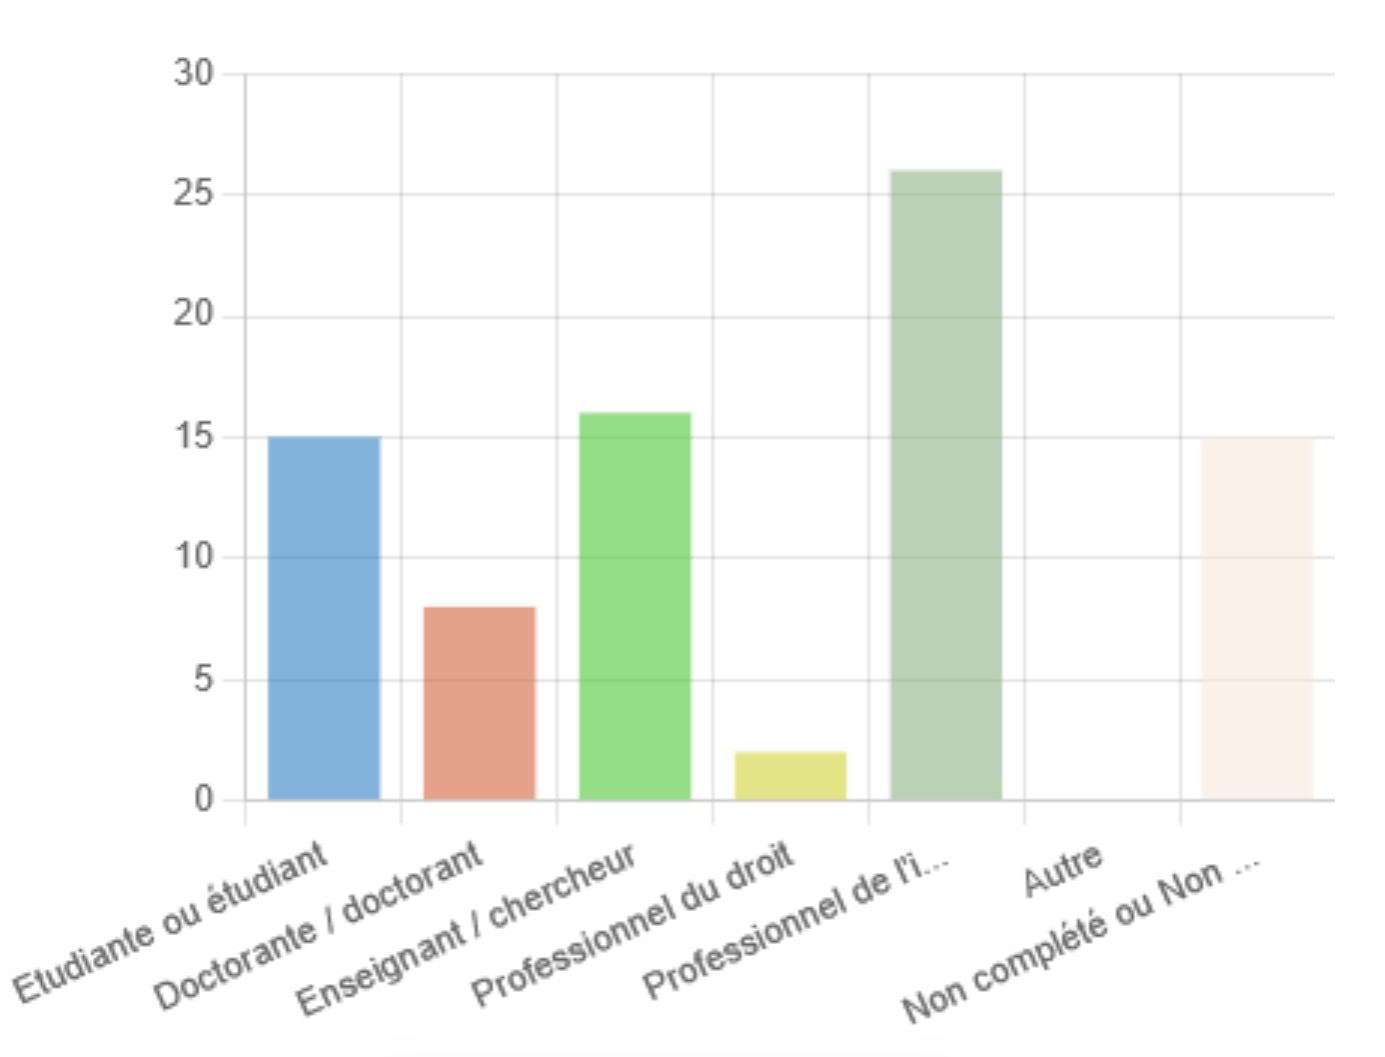
\includegraphics[width=0.5\textwidth]{./images/IMG_5952.jpeg}

Spécialité des lecteurs : 

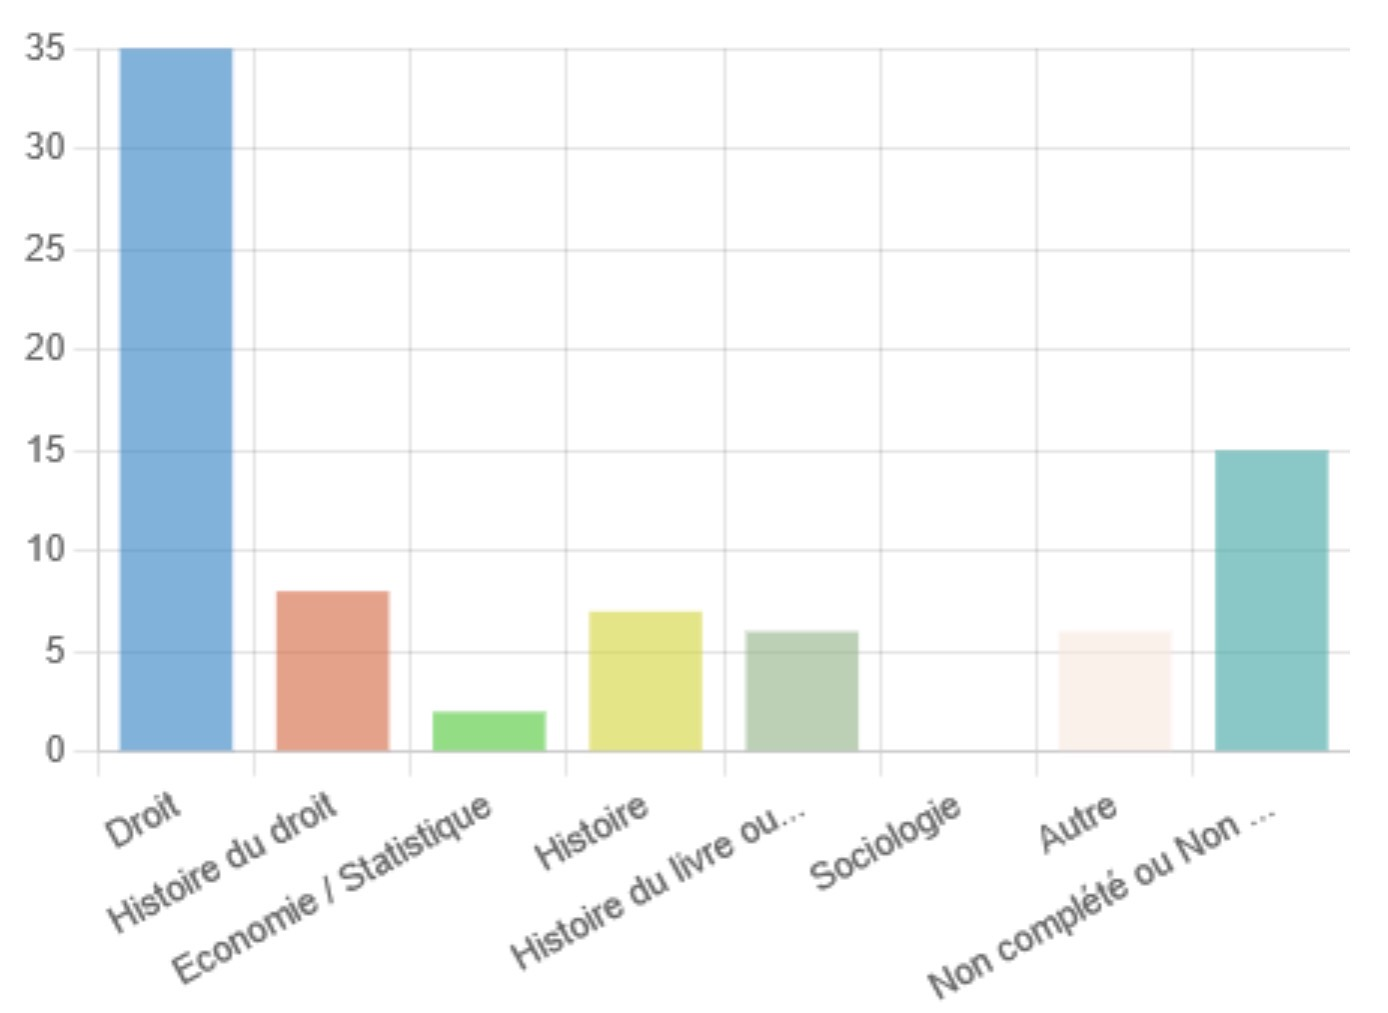
\includegraphics[width=0.5\textwidth]{./images/IMG_5953.jpeg}

Réponses aux nouveaux services ou fonctionnalités proposées :  

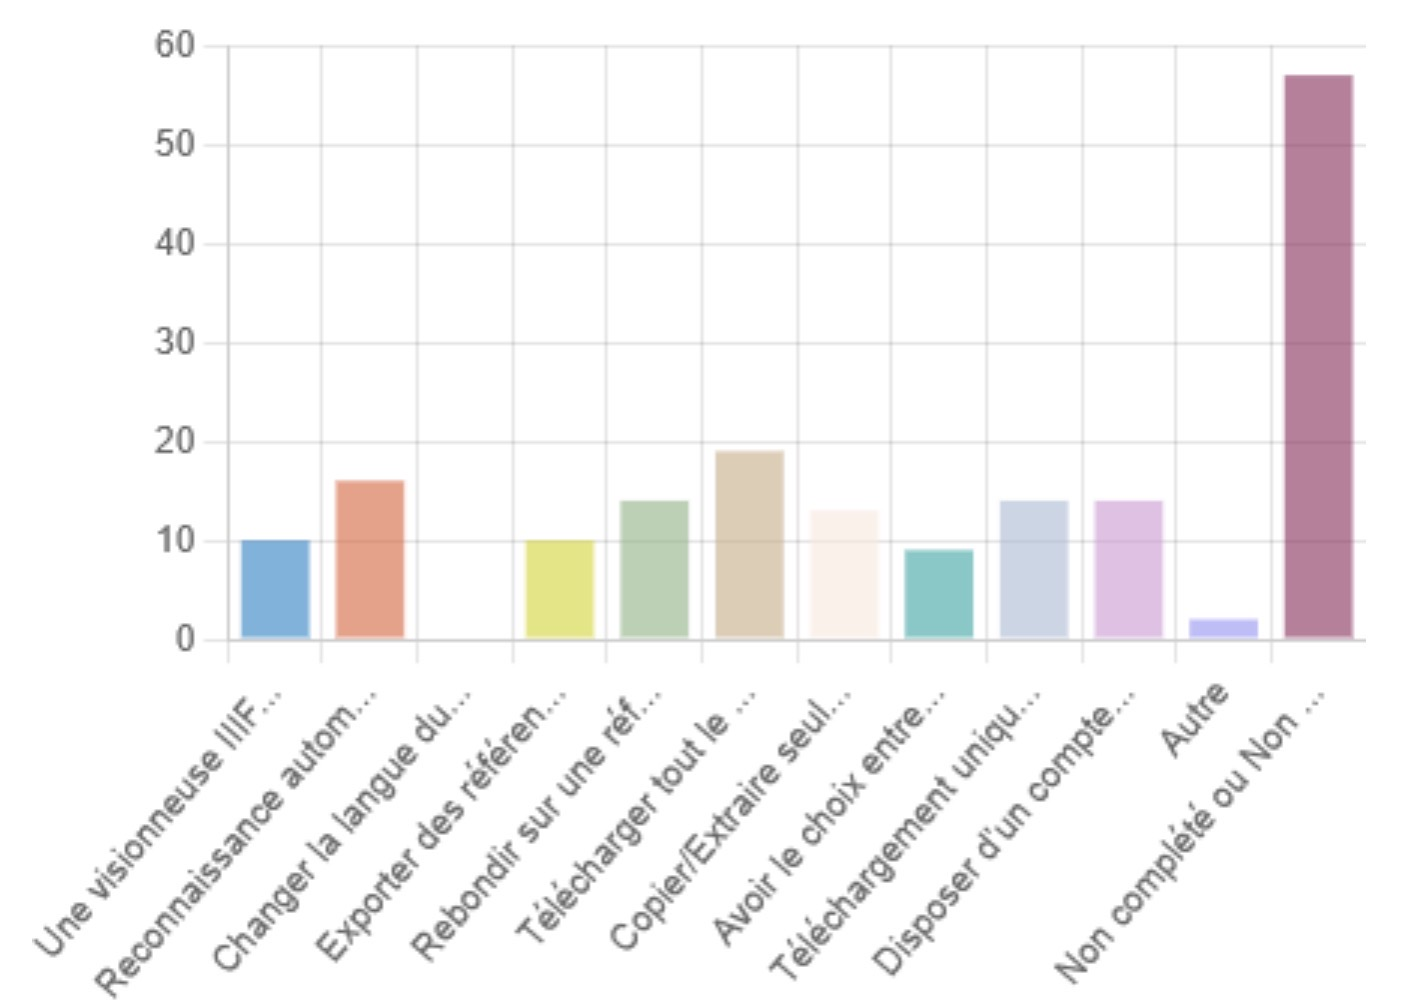
\includegraphics[width=0.5\textwidth]{./images/IMG_5954.jpeg}

